% Author: Mathias Hablützel

\section{Erfassung Schiffsgeschwindigkeiten}

\subsection{Problemanalyse}
\subsubsection{Windangriffswinkel und Windgeschwindigkeit}

\begin{wrapfigure}{r}{6cm} 
\centering
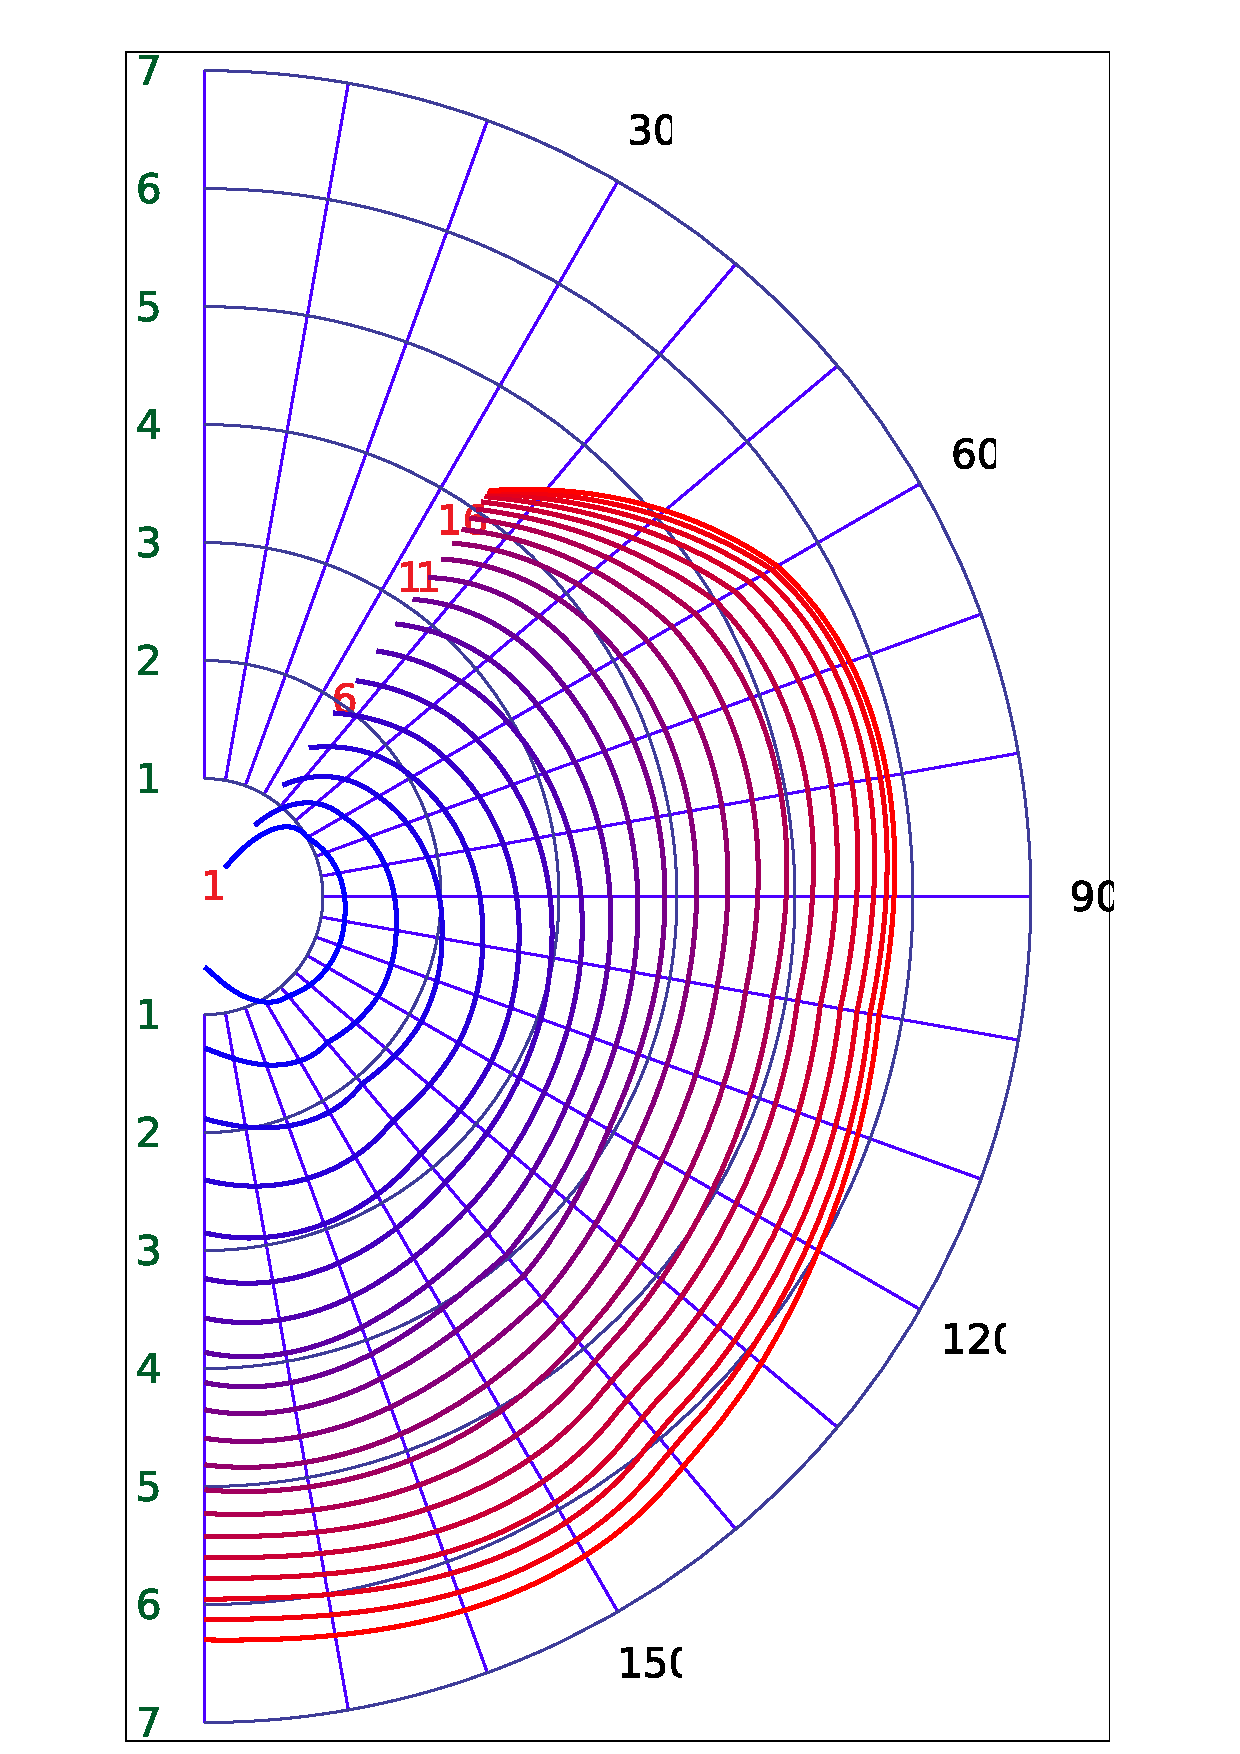
\includegraphics[width=6cm]{img/polardiagramm}
\caption{Polardiagramm eines Bootes, grün Windstärke in Knoten, rot
Geschwindigkeit in Knoten, schwarz Windangriffswinkel}
\label{polardiagram}
\end{wrapfigure}

Je nach Einfallswinkel des Windes variert die Schiffsgeschwindigkeit
stark. Bei frontal kommenden Wind fährt das Schiff gar nicht mehr
vorwärts und muss für diesen Umstand aufkreuzen, das heisst einen
Zickzack-Kurs fahren. Deshalb muss für jedes Schiff empirisch der
minimale Einfallswinkels vom Bug aus ermittelt werden, somit ist der
steilste Winkel bekannt.

Die Schiffsgeschwindigkeit variert aufgrund der physischen Eigenschaften
von Segel, Rumpf und Aerodynamik. Entgegen Intuition ist Wind von
Achtern nicht der schnellste, sondern bei sogenannt halben Wind (meist
zwischen 80\degree und 105\degree). Da sich diese Daten nicht nur bei
unterschiedlichen Einfallswinkel verändern, sondern auch bei
unterschiedlichen Windgeschwindigkeiten, empfiehlt es sich ein
sogenanntes Polardiagramm zu erstellen, dass die unterschiedliche
Fahrtgeschwindigkeiten in Bezug zu Einfallswinkel und
Windgeschwindigkeit darstellt.

Da aber der Datensatz nicht durchgehend ist, muss zwischen den bekannten
und ermittelten Punkten interpoliert werden.

\subsubsection{Interpolationsverfahren}
Um diese Daten zu interpolieren eignet sich die bilineare Interpolation
am besten, da sie sehr einfach zu implementieren ist, über eine für
unsere Zwecke genügend hohe Genauigkeit verfügt, in linearer Zeit
rechnet und nur aus Multiplikationen sowie Additionen besteht, was
aufgrund von den heutigen CPU-Befehlen nur noch wenigen Taktzyklen
braucht und somit zu einer sehr hohen Ausführgeschwindigkeit führt.

Andere Interpolationsmethoden wie qubische Interpolation,
Spline-Interpolation oder polynomielle Interpolation sind entweder zu
ressourcen konsumierend, langsam oder sogar instabil. Daher wurde diese
nicht in Betracht gezogen. Ausserdem verwendet dieses Verfahren nur die
unmittelbaren Nachbarwerte und kommt damit mit weniger Informationen
zurecht.

\subsection{Implementation}
\subsubsection{Eingabedaten-Parser}
Die Schiffsdaten sind als CSV\footnote{Comma Separated Values}-Datei
gegeben und werden von einem selbst\-geschriebenen Parser in ein
passendes Klassen-Konstrukt geladen. Die Schwierigkeit bestand darin,
dass die Daten nicht-dekoriert sind und daher nur durch ihre Position
von anderen Typen zu unterscheiden sind. Das bedeutet allerdings auch,
dass der Parser sich auf diese Datenstruktur verlässt und keine
Abweichungen duldet und sonst abstürzt.

Dieses Problem ist allerdings vertretbar, da die Datenstruktur
vorgegeben ist und der Parser daran angepasst wurde.

\subsubsection{Verarbeitungsklasse}
Die Klasse \texttt{BoatSpeedDiagram.java\footnote{Im Package 
ch.zhaw.lakerouting.interpolation.boatdiagram zu finden}} verwaltet das
Polardiagram und bietet die nötigen Methoden für die Abfrage der Werte
an, kapselt die Interpolation, so das der Programmierer sich darum nicht
kümmern muss.

\subsubsection{Bilineare Interpolation}\label{sss:bilinearinterpolation}
Die Interpolation an sich ist durch 
\begin{equation}
f(x,y) \approx \begin{bmatrix} 1-x & x \end{bmatrix} \begin{bmatrix}
f(0,0) & f(0,1) \\ f(1,0) & f(1,1) \end{bmatrix} \begin{bmatrix} 1 - y
\\ y \end{bmatrix}
\label{eq:bilineareinterpolation}
\end{equation}
geben und kann in Java wie nachfolgend gezeigt, implementiert werden.

 \lstinputlisting[label=src:bilinearinterpolation,caption=Bilineare Interpolation]{code/BilinearInterpolation.java}
Die konkrete Berechnung erfolgt auf den Zeilen 17-19 und zeigen den
einfachen Charakter der Berechnung. Diese Implementation erfordert
allerdings eine geringe Aufbereitung der Eingabewerte, ist dafür
einfacher zu testen und somit indirekt auch weniger anfällig für
Implementationsfehler, was direkt zu robusterem Code führt.
